%----------------------------------------------------------------------------------------
%    PACKAGES AND THEMES
%----------------------------------------------------------------------------------------
\documentclass[aspectratio=169,xcolor=dvipsnames]{beamer}
\makeatletter
\def\input@path{{theme/}}
\makeatother
\usetheme{CleanEasy}
\usepackage[utf8]{inputenc}
\usepackage{lmodern}
\usepackage[T1]{fontenc}
% \usepackage[brazil]{babel}
\usepackage{fix-cm}
\usepackage{amsmath}
\usepackage{mathtools}
\usepackage{listings}
\usepackage{xcolor}
\usepackage{hyperref}
\usepackage{caption}
\usepackage{graphicx} % Allows including images
\usepackage{booktabs} % Allows the use of \toprule, \midrule and \bottomrule in tables
\usepackage{tikz}
\usetikzlibrary{positioning, shapes, arrows, calc, decorations.pathreplacing, arrows.meta, backgrounds, patterns, overlay-beamer-styles}
\usepackage{etoolbox}
\usepackage{animate}

%----------------------------------------------------------------------------------------
%    LAYOUT CONFIGURATION
%----------------------------------------------------------------------------------------
% Configure code listings
\lstset{
  basicstyle=\ttfamily\small,
  keywordstyle=\color{blue},
  commentstyle=\color{green!60!black},
  stringstyle=\color{red},
  showstringspaces=false,
  breaklines=true,
  frame=single,
  rulecolor=\color{black!30},
  backgroundcolor=\color{black!5},
  numbers=left,
  numberstyle=\tiny\color{black!70},
  numbersep=5pt
}

%----------------------------------------------------------------------------------------
%    TITLE PAGE
%----------------------------------------------------------------------------------------


%---------------------------------------------


\title[Nice Title]{X-ray Characterization of Aerogel Foams: Quantifying When Scattering Effects Require Corrections for Accurate Density Measurement}

\author[A. Name]{Yuegelica Yeong\inst{1} \and Pawel M. Kozlowski}

\institute[VFU]{\inst{1}%
  Institute for Computing in Research\\
}


\vspace{-2cm}\date{\today}
% Define positions for logos on title page
\titlegraphic{
  \begin{tikzpicture}[remember picture, overlay]
  \end{tikzpicture}
}


%----------------------------------------------------------------------------------------


\begin{document}

\begin{frame}[plain]
  \titlepage
\end{frame}

\begin{frame}{What are aerogels?}
\begin{itemize}
  \item Lightest solid material
  \item Amazing insulators
  \item High Porosity, low density
\end{itemize}
 \begin{figure}[h!]
    \centering
    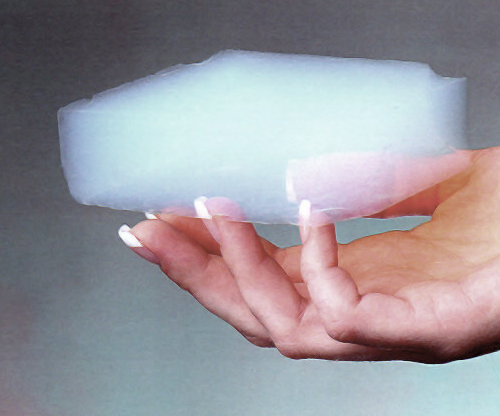
\includegraphics[width=0.29\textwidth]{aerogel.png}
  \end{figure}
\end{frame}

\begin{frame}{High Energy Density Physics}
Extreme conditions!
\begin{itemize}
  \item Astrophysics
  \item Shielding Tech
  \item Inertial Confinement Fusion (ICF)
  \item Nuclear Detonation
\end{itemize}
 \begin{figure}[h!]
    \centering
    \includegraphics[width=0.29\textwidth]{supernovae.png}
  \end{figure}
\end{frame}


\begin{frame}{Motivation: Foam Densities set the initial X-ray speed}
\begin{itemize}
  \item Aerogels as radiative targets
  \item Vaporized during the shot.
  \item Beer-Lambert law to estimate density.
\end{itemize}
 \begin{figure}[h!]
    \centering
    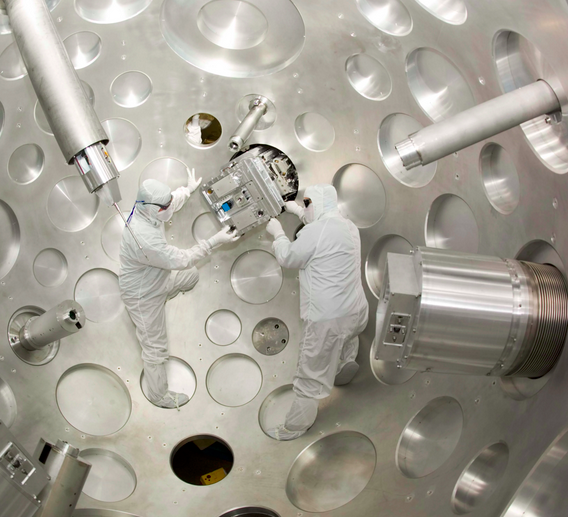
\includegraphics[width=0.29\textwidth]{omega.png}
  \end{figure}
\end{frame}

\begin{frame}{Radiation Flows}
\begin{itemize}
  \item Lasers hit gold halfrum -> radiation flow
  \item Radiation shocks push material forward -> Radiation front
\end{itemize}
 \begin{figure}[h!]
    \centering
    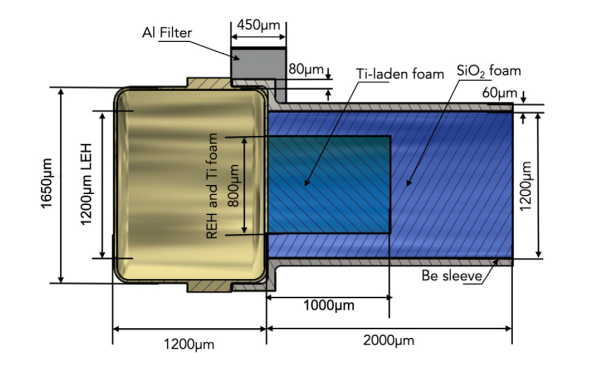
\includegraphics[width=0.35\textwidth]{holfrum.png}
  \end{figure}
\end{frame}

\begin{frame}{OMEGA-60 and Shock Fronts}
    \begin{minipage}{0.48\textwidth}
  \centering
  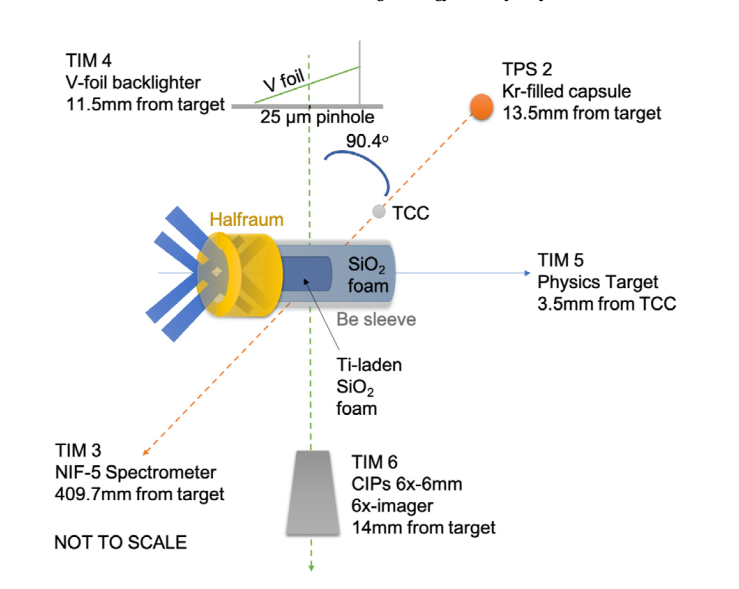
\includegraphics[width=\textwidth]{coaxplatform.png}
\end{minipage}
\hfill
\begin{minipage}{0.48\textwidth}
  \centering
  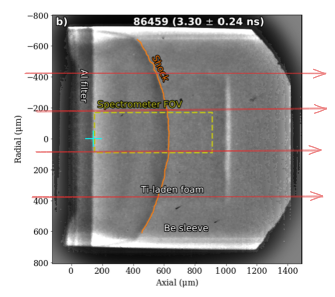
\includegraphics[width=\textwidth]{coax3anew.png}
\end{minipage}
\end{frame}

\begin{frame}{Research Question}
  \begin{block}{Main Research Question}
    When are \textbf{scattering effects} large enough to bias density estimates from Beer-Lambert Law beyond experimental tolerances?
  \end{block}

\end{frame}


\begin{frame}{Beer-Lambert Law Model}
  \begin{equation*}
    T = \frac{I}{I_0} =e^{-\mu \ell} = e^{\frac{-\mu }{\rho}{\rho}\ell}
  \end{equation*}
  \begin{itemize}
    \item $\mu$: linear attenuation coefficient computed from Henke $f_2$ values
    \item $\ell$: path length (initially assumed to be foam height)
    \item $\frac{\mu}{\rho}$: Mass attenuation coefficient, where $\rho$ is the density.
  \end{itemize}
    \begin{figure}[h!]
    \centering
    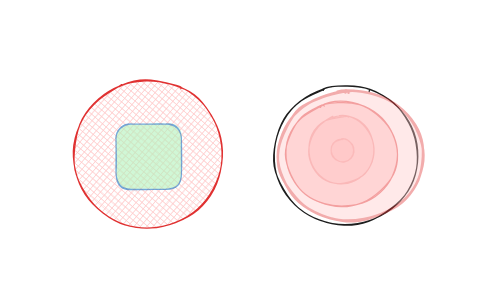
\includegraphics[width=0.29\textwidth]{circular.png}
    \caption{The assumptions of current DCS measurements}
  \end{figure}
\end{frame}

\begin{frame}{Transmission and Intensity}
      \begin{figure}[h!]
    \centering
    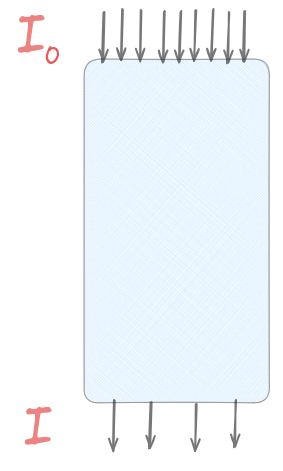
\includegraphics[width=0.295\textwidth]{intensity.png}
  \end{figure}
\end{frame}
\begin{frame}{Experimental Setup}
\begin{minipage}{0.32\textwidth}
  \centering
  \small
  \captionof{table}{Foam and Imaging Parameters}
  \begin{tabular}{ll}
    \toprule
    \textbf{Property} & \textbf{Value} \\
    \midrule
    Foam Composition & (SiO$_2$)$_5$ + Ti \\
    Pore Radius & 1 $\mu$m \\
    Porosity & 98.5\% \\
    Required Accuracy & $\pm$2 mg/cc \\
    \bottomrule
  \end{tabular}
\end{minipage}
\hfill
\begin{minipage}{0.32\textwidth}
  \centering
  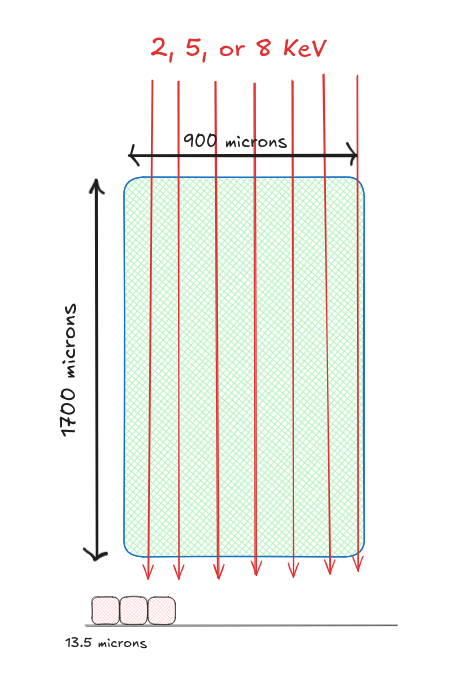
\includegraphics[width=\textwidth]{foamimagingparameters.png}
\end{minipage}
\end{frame}


\begin{frame}{Verifying Beer-Lambert}
  \begin{figure}[h!]
    \centering
    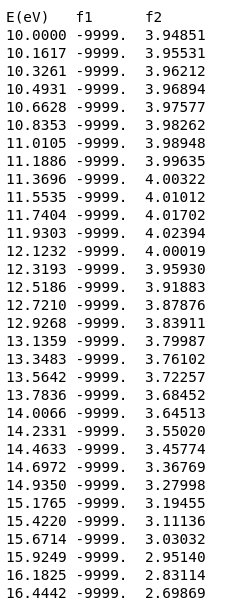
\includegraphics[width=0.295\textwidth]{Screenshot 2025-07-30 at 19-29-12 .png}
    \caption{File for the element $Si$ provided from Henke}
  \end{figure}
We used a weight fraction of each elemtn by computing the molar mass (mendeleev) and the mass attenuation.
The arrays from the Henke files had a different number of energy values, so interp
\end{frame}

\begin{frame}{Transmission vs Energy}
  \begin{figure}[h!]
    \centering
    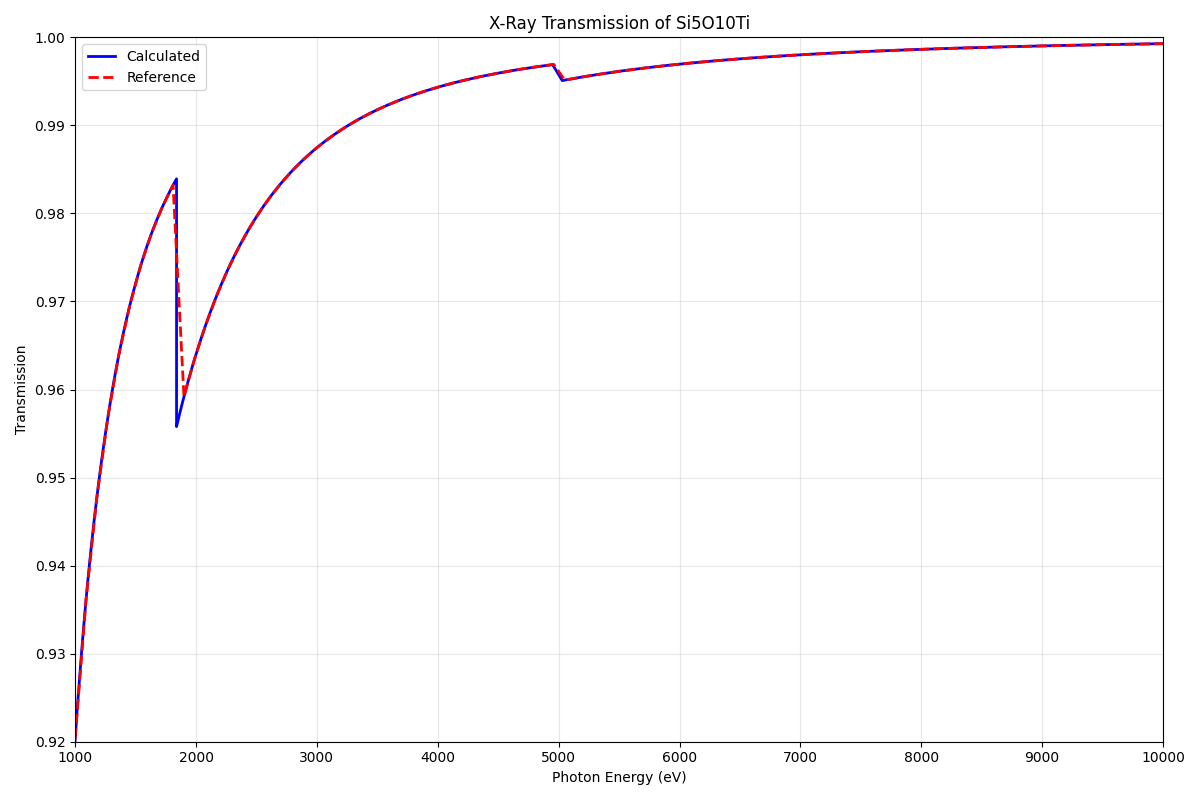
\includegraphics[width=0.6\textwidth]{energy_vs_transmission.png}
    \caption{Transmission vs Photon Energy for $(SiO_2)_5 + Ti$ foam with a density of $2.33 \frac{g}{cm^3}$ and a path length $(\ell)$ of $0.1 \mu m$. General increasing trend because the X-rays penetrate the material easier.}
  \end{figure}
\end{frame}


\begin{frame}{Simulation Workflow}
  \begin{enumerate}
    \item Compute $\mu$ from material and photon energy
    \item Simulation of photons that hit the pores at random distances from center
    \item Refraction using Snell's Law at each pore
    \item Calculate total path length per photon
    \item Apply Beer-Lambert attenuation
    \item Bin resulting intensities on CCD
\end{enumerate}
\end{frame}


\begin{frame}{Important Equations}
\begin{itemize}
  \item \textbf{Attenuation Coefficient}
  \[
    \mu = \frac{\rho N_A}{M_A} \cdot 2 r_e \lambda f_2
  \]
  \item \textbf{Snell's Law for Refraction:}
  \[
    n_1 \sin\theta_i = n_2 \sin\theta_t
  \]
  \item \textbf{Average Number of Pore Interactions:}
  \[
    N_{\text{pore interactions}} = \frac{\text{Foam Height}}{\text{Mean Free Path}}
  \]
\end{itemize}

\end{frame}

\begin{frame}{Effects of Scattering}
  \begin{figure}[h!]
    \centering
    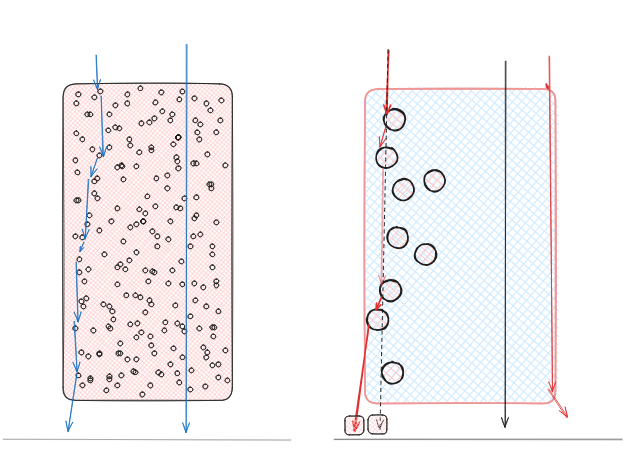
\includegraphics[width=0.6\textwidth]{sidebyside.png}
    \caption{Horizontal displacement caused by interactions with pores.}
  \end{figure}

\end{frame}
\begin{frame}{Computing Lateral Displacement}
\centering
To compute lateral displacement, we track $\Delta{x}, \Delta{\theta_i}$.
\[\Delta{x}=\sqrt{2r^2(1-\cos({180-2\theta_r))}}\]

\hspace*{0.1\textwidth} % push images towards center
\begin{minipage}{0.25\textwidth}
  \centering
  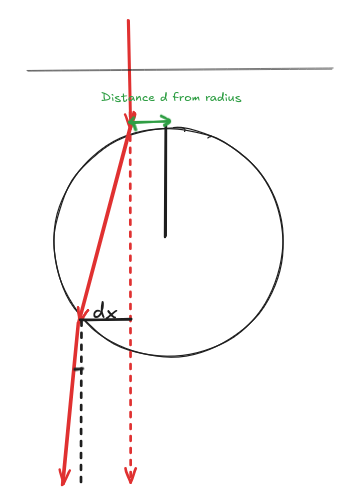
\includegraphics[width=\linewidth]{zoomedindx.png}
\end{minipage}
\hspace{0.05\textwidth}
\begin{minipage}{0.2\textwidth}
  \centering
  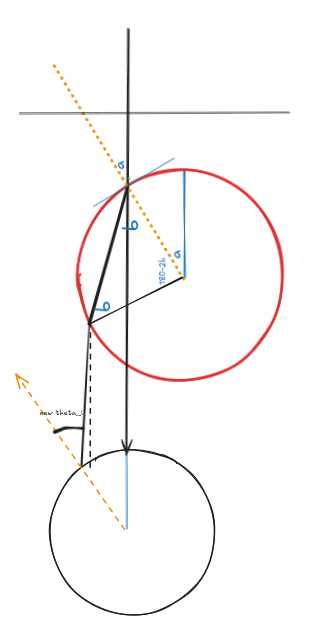
\includegraphics[width=\linewidth]{incidenceangle.png}
\end{minipage}
\end{frame}
\begin{frame}{Horizontal Displacement}
      \begin{figure}[h!]
    \centering
    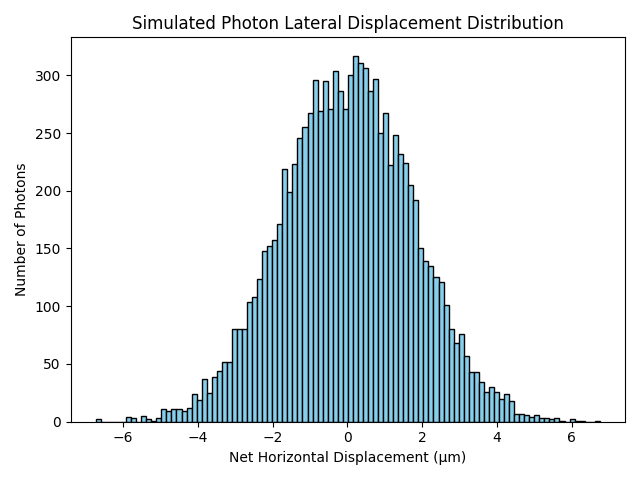
\includegraphics[width=0.6\textwidth]{lateral_displacement.png}
    \caption{Lateral Displacement caused by refraction due to Snell's law.}
  \end{figure}
\end{frame}


\begin{frame}{Path Length and Net Intensity}
\begin{itemize}
    \item Path length computed via Pythagorean theorem.
    \item Transmission summed per CCD pixel. Greater deflection reduces intensity.
\end{itemize}

\vspace{-0.2cm} % move image block upward

\begin{center}
\begin{minipage}{0.3\textwidth}
  \centering
  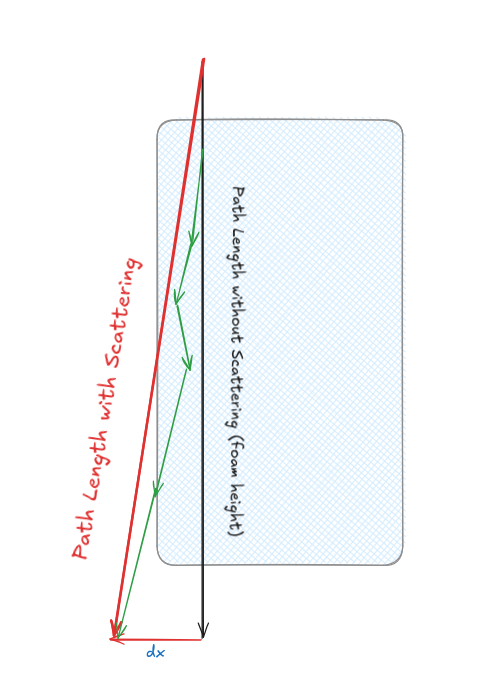
\includegraphics[width=\linewidth]{pathlength.png}
\end{minipage}
\hspace{0.05\textwidth}
\begin{minipage}{0.4\textwidth}
  \centering
  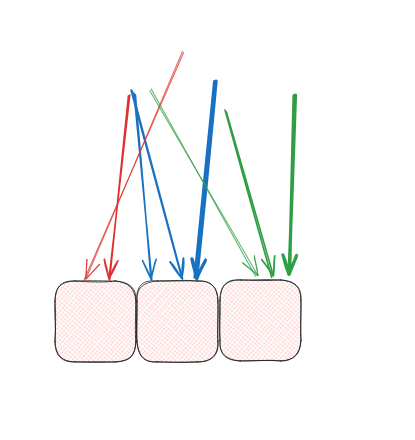
\includegraphics[width=\linewidth]{netintensity.png}
\end{minipage}
\end{center}
\end{frame}



\begin{frame}{Transmission Difference Due to Scattering}
  \begin{figure}[h!]
    \centering
    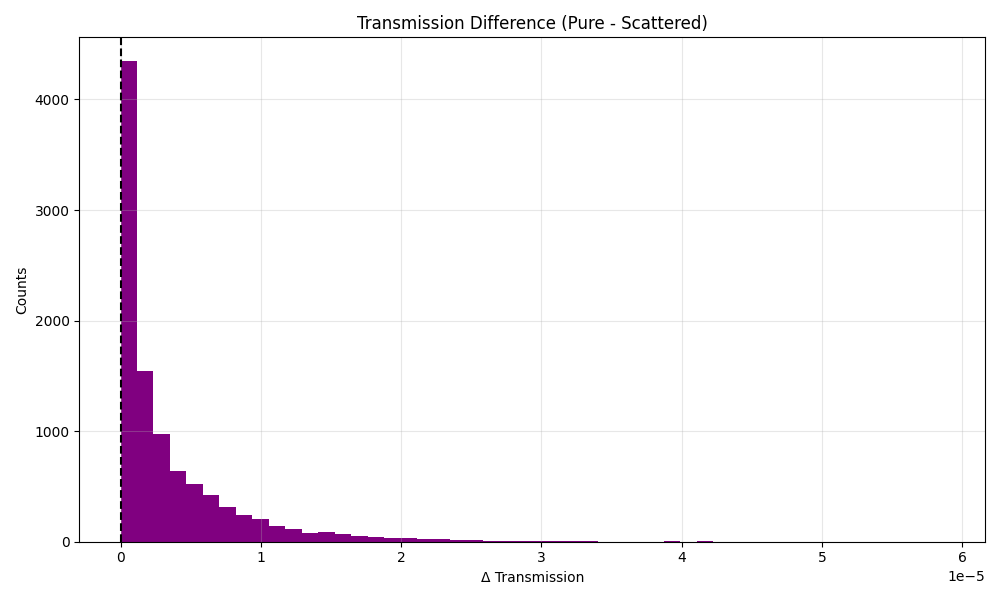
\includegraphics[width=0.6\textwidth]{transmission_diff.png}
    \caption{Transmission across foam with vs. without scattering. Average percent difference of $2.96 \times10^{-6}$.}
  \end{figure}

\end{frame}


\begin{frame}{CCD Intensity Distribution}
  \begin{figure}[h!]
    \centering
    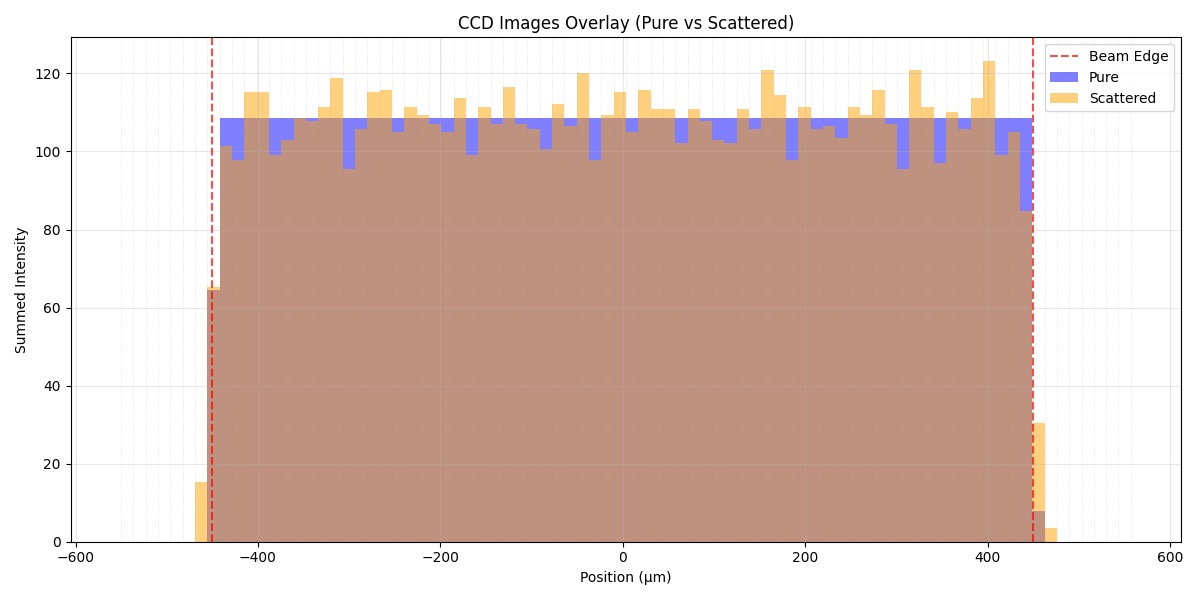
\includegraphics[width=0.8\textwidth]{CCD_Overlay_new.png}
    \caption{Simulated CCD intensity profile. Summed intensity binned to match $13.5\,\mu m$ pixel resolution.}
  \end{figure}
\end{frame}

\begin{frame}{Zoomed-in Foam Edge: Left and Right}
  \begin{columns}
    \column{0.48\textwidth}
    \centering
    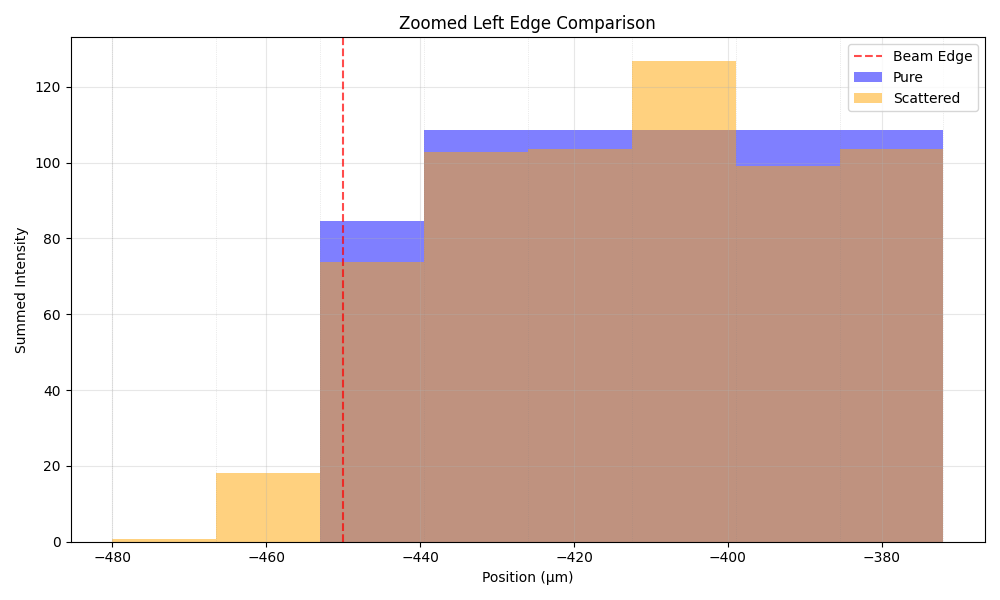
\includegraphics[width=\linewidth]{zoomed_left_edge_new.png}
    \captionof{figure}{Zoomed view: Left edge intensity}
    
    \column{0.48\textwidth}
    \centering
    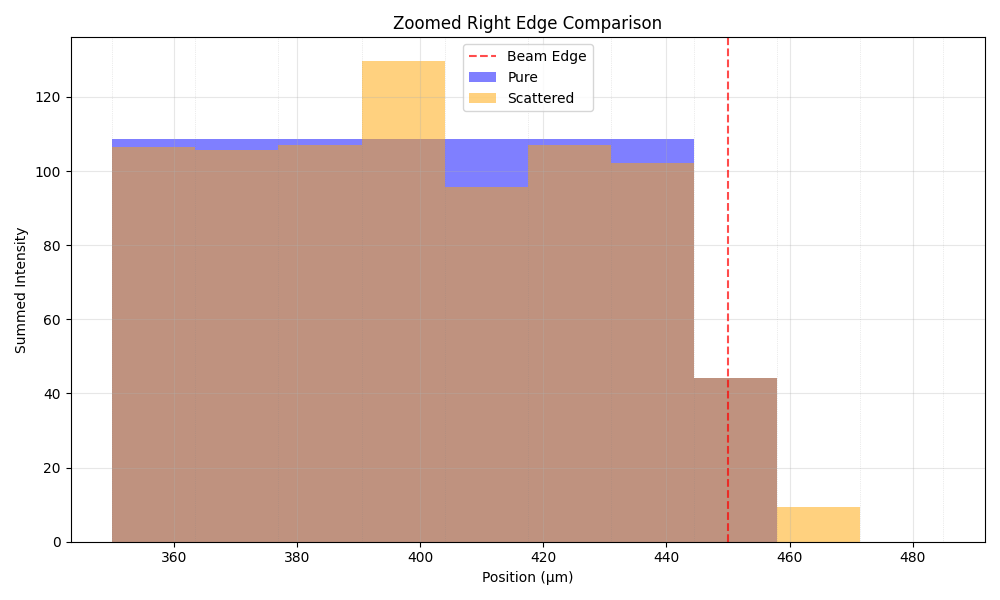
\includegraphics[width=\linewidth]{zoomed_right_edge_new.png}
    \captionof{figure}{Zoomed view: Right edge intensity}
  \end{columns}
  \vspace{0.3cm}
  \begin{block}{Observation}
    There is a notable effect on Transmission by scattering caused by refraction.
  \end{block}
\end{frame}


\begin{frame}{Scattering vs Measurement Tolerance}
  \begin{itemize}
    \item The CCD sensor has noise levels of a few percent.
    \item A deviation \textless 2–3\% is within tolerance.
\[
\text{Percent Difference} = \left| \frac{I_{\text{scattered}} - I_{\text{pure}}}{I_{\text{pure}}} \right| \times 100\%\]

  \end{itemize}
\end{frame}

\begin{frame}{Pore Size and Porosity}
To simulate realistic foam densities between 25--100 mg/cc, we computed the required pore volume fractions assuming a solid density of $2.2$ g/cc.

\begin{table}[h!]
\centering
\begin{tabular}{ccc}
\toprule
\textbf{Density} & \textbf{Unit} & \textbf{Pore Volume Fraction $\phi$} \\
\midrule
100 & mg/cc & 0.955 \\
66  & mg/cc & 0.970 \\
44  & mg/cc & 0.980 \\
22  & mg/cc & 0.990 \\
\bottomrule
\end{tabular}

\end{table}

\begin{block}{Porosities Used}
    $[50, 60, 70, 80, 90, 95] \%$
\end{block}

\begin{block}{Pore Sizes Used}
$[10^{-7}, 10^{-6}, 10^{-5}, 3 \cdot 10^{-5}, 10^{-4}]$ cm
\end{block}
    
\end{frame}

\begin{frame}{Absolute Horizontal Displacement as a function of pore size and porosity}
  \begin{columns}
    \column{0.48\textwidth}
    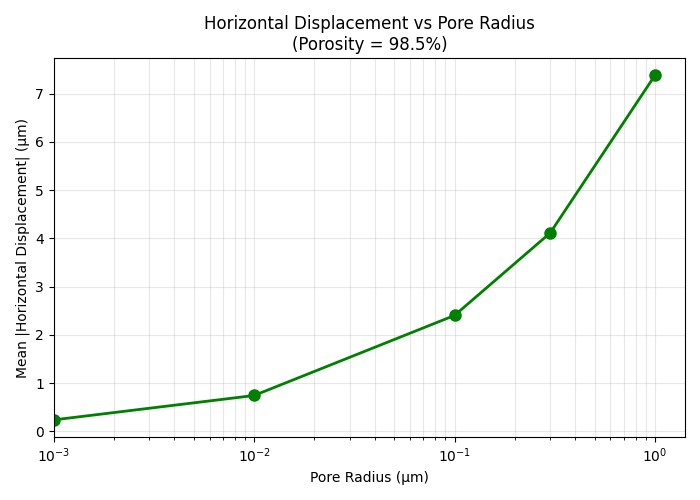
\includegraphics[width=\textwidth]{dxvsporeradiusnew.png}
    \captionof{figure}{Mean $\Delta x$ vs Pore Size}
    \column{0.48\textwidth}
    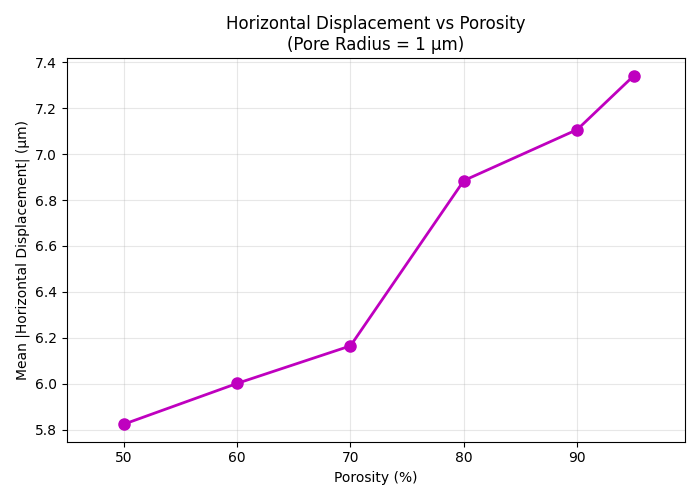
\includegraphics[width=\textwidth]{dxvsporositynew.png}
    \captionof{figure}{Mean $\Delta x$ vs Volume Fraction}
  \end{columns}
\end{frame}

\begin{frame}{Intensity Ratio as a function of pore size and porosity}
  \begin{columns}
    \column{0.48\textwidth}
    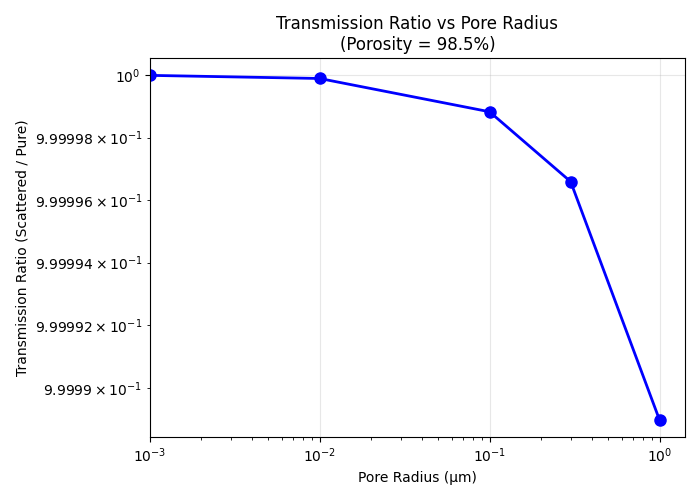
\includegraphics[width=\textwidth]{transmissionvspore1.png}
    \captionof{figure}{Transmission Ratio vs Pore Size}
    \column{0.48\textwidth}
    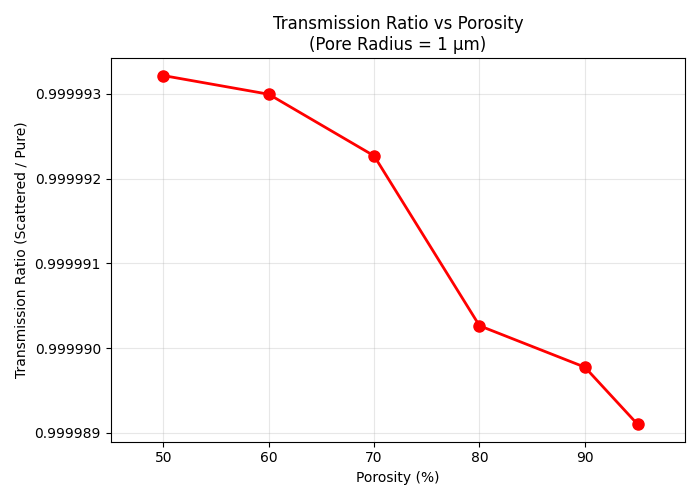
\includegraphics[width=\textwidth]{transmissionvsporosity1.png}
    \captionof{figure}{Transmission Ratio vs Volume Fraction}
  \end{columns}
\end{frame}


\begin{frame}{Discussion and Conclusions}
\begin{block}{Key Insight}
  Larger pores and higher porosity lead to greater deviation from ideal attenuation, increasing error in inferred density.
\end{block}
\begin{block}{Key Insight}
    Percievable scattering effect due to refraction. Larger pore radii increased the effect.
\end{block}
\begin{block}{Key Insight}
    No significant scattering effect caused by longer path. $\Delta{T}\leq 1\text{e}^{-6}$, which is negligible.
\end{block}

\end{frame}

\begin{frame}{Future Work}
  \begin{itemize}
    \item Extend to ray-tracing with explicit geometry
    \item Radiative Transfer Equation (Dynamic model)
  \end{itemize}
\end{frame}

\begin{frame}[plain]
  \centering
  \Huge \textbf{Thank you!}
  
  \vspace{1cm}
  \normalsize
  \href{mailto:your@email.com}{yuegelicay@gmail.com}
  
  \vspace{0.5cm}
  \small
  \texttt{https://github.com/yuegelica/Scattering-EdgeEffects}
\end{frame}

% Sample bibliography (not shown in presentation, just for reference)
%\begin{frame}{References}
%  \begin{thebibliography}{9}
%    \bibitem{einstein1905}
%      Albert Einstein.
    %  \emph{On the Electrodynamics of Moving Bodies}.
 %     Annalen der Physik, 1905.
    
  %  \bibitem{beamer}
 %     Till Tantau.
 %     \emph{The Beamer Class}.
 %     \url{https://ctan.org/pkg/beamer}
 % \end{thebibliography}
%\end{frame}

% \begin{frame}{References}
%   \bibliography{reference.bib}
%   \bibliographystyle{apalike}
% \end{frame}

\end{document}
